\section{Aire Guru}

Urban residents are surrounded by many sources of air pollution, and it is the direct cause of many different symptoms, ranging from simple eye irritation to, in extreme cases, death.
This is particularly true for high-risk groups like children and the elderly.
The WHO (World Health Organization) estimates that there are 4.2 million deaths (https://www.who.int/airpollution/ambient/en/) per year due to air pollution.\\

Air pollution has a significant effect on people with asthma, cardiopathies, allergies, and neurological pathologies.
Air pollution not only aggravates existing diseases, but can also be an initial cause of them, such as in the case of foetal brain damage
(https://www.cronicabalear.es/2018/07/la-contaminacion-ambiental-causa-enfermedades-neurologicas-y-envejecimiento-del-cerebro)
caused by the mother's exposure to air pollution.\\

To be able to control the level of exposure we need to know the levels in the specific locations that we frequent, and the variation during specific times.
To make this information as accessible as possible, it should be freely and publicly available, and the presentation must be simple enough to be understandable by the average citizen.\\

We have created a website - Aire Guru - which collects hourly air pollution measures, stores them for historical use, 
processes them to extract relevant information, personalizes them to engage the user with regard to their individual
circumstance, visualizes them in an easy to understand format, and provides them online to facilitate its accessibility, free of charge.
Furthermore, descriptions of all the data and how it has been processed are also provided to raise public awareness of the value of this data.
Aire Guru has been successfully tested, using the Air Quality data provided by the Málaga open data portal(https://datosabiertos.malaga.eu/) in the Spanish city of Málaga.\\

There are some online data sources already available, however they have various failings.
The most common problems are:

\begin{itemize}

    \item Obsolete measurements. Measurements need to be taken regularly, since there can be huge differences
          between pollution levels at different times of the day.

    \item Limited geographic coverage. The data must cover a reasonable proportion of areas that people spend significant time in.

    \item Insufficiently granular measurements. Measurements must be at a reasonably fine level of granularity. One single measurement for an entire city is not useful.

    \item Poor presentation. Often the information is presented in an uninterpreted form, making it difficult for users to visualize, especially in a geographic sense.

    \item Poor discrimination and interpretation. Many tools show individual values as a number or a colour. This information is not
          enough for the user to take control of their exposure. Such visualizations are not really compelling. 

\end{itemize}

Our website solves the deficiencies described above.\\

Measurements are published hourly and come from measurement stations placed throughout the 
city of Málaga, covering entire urban region at a granularity of $100m^2$.\\

The information is presented in a clear and simple manner, making it possible to see the most polluted regions, and allowing the user to make comparisons both geographically and historically.
It provides personalised information, such as the most relevant pollutants for a user's particular medical conditions, and can track
the pollution they are exposed to both in real time and over a historical period, by linking with location data from their mobile device. \\

While building Aire Guru we were confronted with the following challenges:\\

As mentioned before, the data is provided on the Malaga's open data portal.
This is not a intuitive place to search for air pollution information for the average user.
Aire Guru provides the information in a way that is easier for the user - in a browser.\\

The data offered in the open data portal is in GeoJSON format.
This format is highly structured and easy to process given the appropriate software expertise. It is not usable by the general public in this form however.
The data model contains multiple readings of different kinds, such as qualitative and quantitative measurements from fixed and mobile sensors.
Different sensors provide different sets of fields.
Aire Guru is able to process all of them and offer the user an unified vision of the measurements offered by all the stations.\\

The Aire Guru data collection and transformation pipeline is fully automated, and runs without any human intervention or management.
The sensors provide hourly data, and the Aire Guru interface reflects this granularity, represent the data with the same periodicity.
Aire Guru translate the raw sensor data into understandable, useful, actionable information, using graphs, icons, colours and text. 
It enables the user to easily visualize the pollution in a specific area, both at the current time and historically. We maintain
a historical log of data, so that the user is able to visualize the evolution of pollutants since 2018. The user can also track their personal exposure
to these pollutants over the same period of time either by enabling location tracking on their mobile device, or by importing their own location
data. Finally, Aire Guru presents information about the health consequences of pollution exposure, and all data can be viewed through this lens.\\

\begin{figure}[ht]
    \centering
    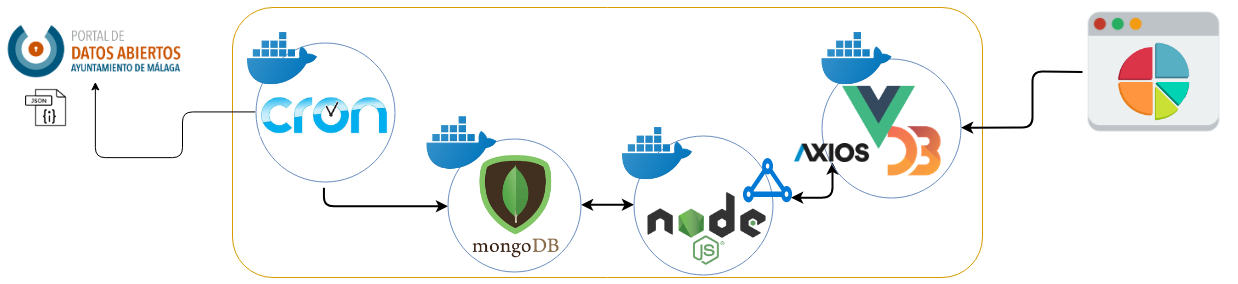
\includegraphics[width=12cm]{Figure_2_1_aireGuruArquitecture}
    \caption{Architecture of Aire Guru}
\end{figure}

\begin{center}
    \bf Figure 2.1. Architecture of Aire Guru\\
\end{center}

\begin{figure}[ht]
    \centering
    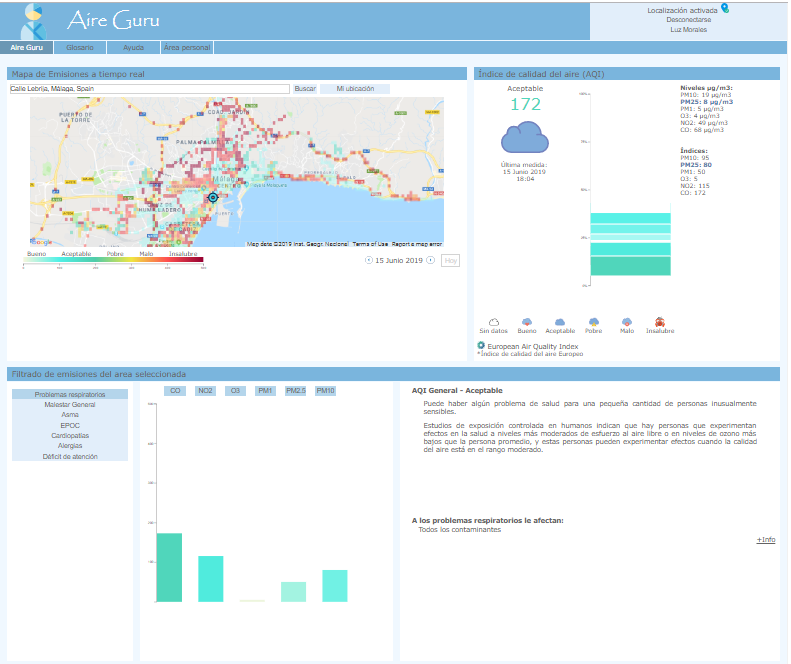
\includegraphics[width=9cm]{Figure_2_2_aireGuru_webInterface}
    \caption{Aire Guru Web Interface}
\end{figure}

\begin{center}
    \bf Figure 2.2. Aire Guru Web Interface\\
\end{center}

To enable access by the majority of the population, Aire Guru is available at the web addresses https://www.aire.guru and https://www.airquality.guru.
We use SSL that guarantees the encryption of data through the network and guarantees access as more and more browsers protect 
users by only showing pages that use a secure transport.\\

As previously mentioned, all users can see the basic information without having to provide any data or identify themselves, and without the need to
perform downloads or installations. Today, almost everyone is familiar with web browsing and we do not force the user to perform extra steps, such as 
requiring them to sign in or install extra software.\\

\subsection*{Evaluation}

The system has been successfully tested with 14 subject in the Spanish city of Málaga. The survey showed a high degree of satisfaction, 
particularly regarding the clarity and completeness of the the information and analysis.\\

After a week, test users completed a survey that contained questions about how understandable the information was
and how useable it was. Additionally, respondants could make their own comments.\\

Most of the respondents agreed that the functionality they liked the most, was to see the air quality index actually in the
map, and suggested increasing the number of zones.
92 \% of the respondents found the information useful and complete, and 71.43 \% answered that they also found it
understandable.\\

More than half of the respondents admit that they did not know the meaning of the air quality index, but after
using the website, they now understand it.\\

Regarding their interest about air quality, half of them indicated that they had never sought information about it,
only two were previously well informed, and one of them marked the 'other' option and specified that using the application had aroused their interest.
In addition, four of them indicated that, thanks to the website, they have now discovered they have a medical condition that is affected by air quality.\\

Among the test subjects, a greater awareness of pollution has been recognized, and they now show more interest in the
air quality in the city and its possible effects on their health.

\begin{figure}[ht]
   \centering
   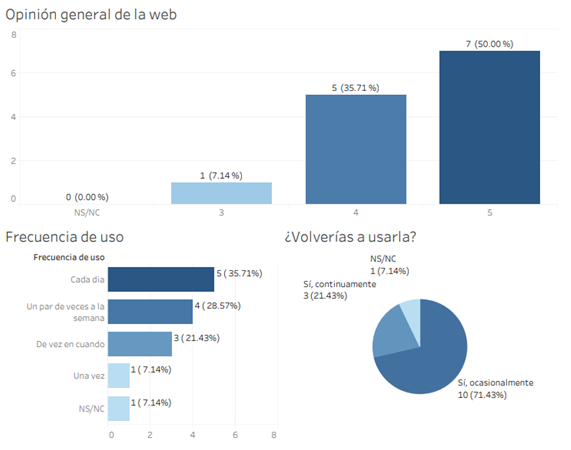
\includegraphics[width=12cm]{Figure_2_3_aireGuruSurveyResults}
   \caption{Aire Guru. Survey results}
\end{figure}

\begin{center}
   \bf Figure 2.3. Aire Guru. Survey results\\
   \end{center}